\title{Study Guide for Midterm 2}
\author{Dr. Jordan Hanson - Whittier College Dept. of Physics and Astronomy}
\date{\today}
\documentclass[10pt]{article}
\usepackage[a4paper, total={18cm, 27cm}]{geometry}
\usepackage{outlines}
\usepackage{graphicx}
\begin{document}
\maketitle

\section{Memory Bank}

\begin{enumerate}
\item $\vec{F} = k \frac{q_1 q_2}{r^2}\hat{r}$ ... Coulomb Force
\item $k = 9 \times 10^{9}$ N C$^{-2}$ m$^{2}$ ... Remember $k = 1/(4\pi \epsilon_0)$.
\item $q_e = 1.6 \times 10^{-19}$ C ... Charge of an electron/proton
\item $\vec{F} = q \vec{E}$ ... Electric field and charge
\item $\vec{E}(z) = \frac{\sigma}{\epsilon_0}\hat{z}$ ... Electric field of two oppositely charge planes each with charge density $\sigma$
\item $\epsilon_0 \approx 8.85 \times 10^{-12}$ F/m
\item $dE = \int k dq / r^2$ ... Remember that $dq$ takes the form below
\item $dq = \lambda dx$ ... Linear charge density (C/m)
\item $\vec{E} \cdot \vec{A} = Q_{enc}/\epsilon_0$ ... Gauss' Law, constant electric field over the surface area.
\item $U = q\Delta V$ ... Potential energy and voltage
\item 1 eV: an electron-Volt is the amount of energy one electron gains through 1 V.
\item $V(r) = k\frac{q}{r}$ ... Voltage of a point charge
\item $\vec{E} = -\frac{\Delta V}{\Delta x}$ ... E-field is the slope or change in voltage with respect to distance
\item $V(x) = -E x + V_0$ ... Voltage is linear between two charge planes
\item $Q = CV$ ... Definition of capacitance
\item $C = \frac{\epsilon_0 A}{d}$ ... Capacitance of a parallel plate capacitor
\item $C_{tot}^{-1} = C_1^{-1} + C_2^{-1}$ ... Adding two capacitors \textit{in series.}
\item $C_{tot} = C_1 + C_2$ ... Adding two capacitors \textit{in parallel.}
\item $i(t) = dQ/dt$ ... Definition of current.
\item $v_d = i/(nqA)$ ... Charge drift velocity in a current $i$ in a conductor with number density $n$ and area $A$.
\item $R_{tot}^{-1} = R_1^{-1} + R_2^{-1}$ ... Adding two capacitors \textit{in parallel.}
\item $R_{tot} = R_1 + R_2$ ... Adding two capacitors \textit{in series.}
\item $\Delta V = I R_{\rm tot}$, $\vec{J} = \sigma \vec{E}$ ... Versions of Ohm's Law. ($\vec{J}$ is the current density with units of Amps per meter-squared).
\item $P = I V$ ... Relationship between power, current, and voltage.
\item $V_{\rm C}(t) = \epsilon_1 \left(1 - \exp(-t/\tau)\right)$ ... voltage across the capacitor in an RC series circuit.  The time constant $\tau = RC$.
\item $i(t) = \frac{\epsilon_1}{R} \exp(-t/\tau)$ ... Current in an RC series circuit.
\item $i_{\rm in} = i_{\rm out}$ ... Kirchhoff's junction rule.
\item $\epsilon_1 + \epsilon_2 + \epsilon_3 + ... = 0$ ... Kirchhoff's loop rule.
\item $\vec{F} = a\vec{v} \times \vec{B}$ ... The Lorentz force on a charge $q$ with velocity $\vec{v}$ in a magnetic field $\vec{B}$.
\item $\vec{F} = I\vec{L} \times \vec{B}$ ... The Lorentz force on a conductor of length $\vec{L}$ carrying a current $I$ in a magnetic field $\vec{B}$.
\end{enumerate}

\clearpage

\section{Chapter 9: Current and Resistance}

\begin{enumerate}
\item An ECG monitor must have an RC time constant less than $100 \mu$s to be able to measure variations in voltage over small time intervals. (a) If the resistance of the circuit (due mostly to that of the patient’s chest) is 1.00 k$\Omega$, what is the maximum capacitance of the circuit? (b) Would it be difficult in practice to limit the capacitance to less than the value found in (a)?  (c) If the patient's resistance really is 1.00 k$\Omega$, and the typical maximum amplitude of the patient's heartbeat is 60 mV, when does the voltage rise to 30 mV in the EKG monitor (using the C you found in (a))? \\ \vspace{3cm}
\item Imagine an \textit{alternating current} (AC) system, as opposed to the DC systems we normally consider.  In AC circuits, the voltage follows a form
\begin{equation}
V(t) = V_0 \sin(2\pi f t + \phi)
\end{equation}
The wall outlets in the USA have $f = 60$ Hz and $V_0 = 120$ V.  \textit{We have the freedom to choose $\phi$ in this example, much like choosing the zero-point of voltage.}  (a) Suppose $\phi = 0$.  At what times will $V(t) = 0$? (b) What is the max power delivered to a 1k$\Omega$ resistor? (c) What is the \textit{average} power delivered to a 1k$\Omega$ resistor?  \\ \vspace{3cm} 
\item \textbf{For those of us stuck at home!} A physics student has a single-occupancy dorm room. The student has a small refrigerator that runs with a current of 3.00 A and a voltage of 110 V, a lamp that contains a 100-W bulb, an overhead light with a 60-W bulb, and various other small devices adding up to 3.00 W.  In Southern California, electricity costs about 0.2 dollars per kiloWatt-hour.  How much money does this student spend if the total wattage is on for 12 hours per day for one month? \\ \vspace{2cm}
\end{enumerate}

\section{Chapter 10: Direct-Current (DC) Circuits}

\begin{figure}[ht]
\centering
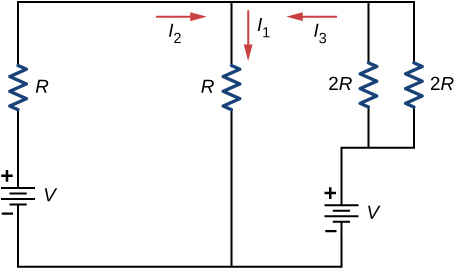
\includegraphics[width=0.35\textwidth]{complexCircuit.jpeg}
\caption{\label{fig:circuit1} A circuit with two batteries and three resistors.}
\end{figure}

\begin{enumerate}
\item Solve for $i_1$, $i_2$, and $i_3$ in Fig. \ref{fig:circuit1}, if $R=1 k\Omega$, and $V = 12.0$ Volts. What power is consumed in the resistors? \\ \vspace{4cm}
\item Suppose an electronic device with resistance $R$ needs between 1.4 and 2.0 volts to operate.  Two AA batteries with $\epsilon = 1.5$V and $r = 0.25\Omega$ are connected (Fig. \ref{fig:ohm2}) in parallel with the device.  (a) If $R = 50\Omega$, what is the current flow? (b) If the batteries each have a charge $q = 2.5$ A hr, how long will the current flow? \\ \vspace{3cm}
\end{enumerate}

\begin{figure}[hb]
\centering
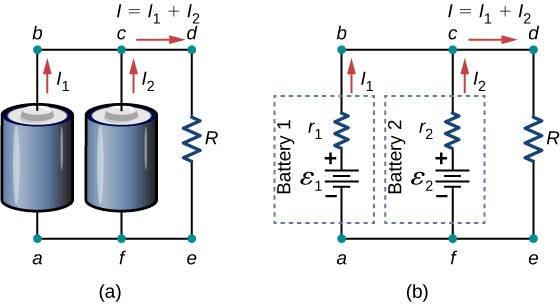
\includegraphics[width=0.45\textwidth]{battery2.jpeg}
\caption{\label{fig:ohm2} Two AA batteries are connected \textit{in parallel} to power a calculator represented by $R$.  (a) The batteries are connected in parallel.  (b) A circuit diagram representing the circuit in (a).}
\end{figure}

\section{Chapter 11: Magnetic Forces and Fields}

\begin{figure}[ht]
\centering
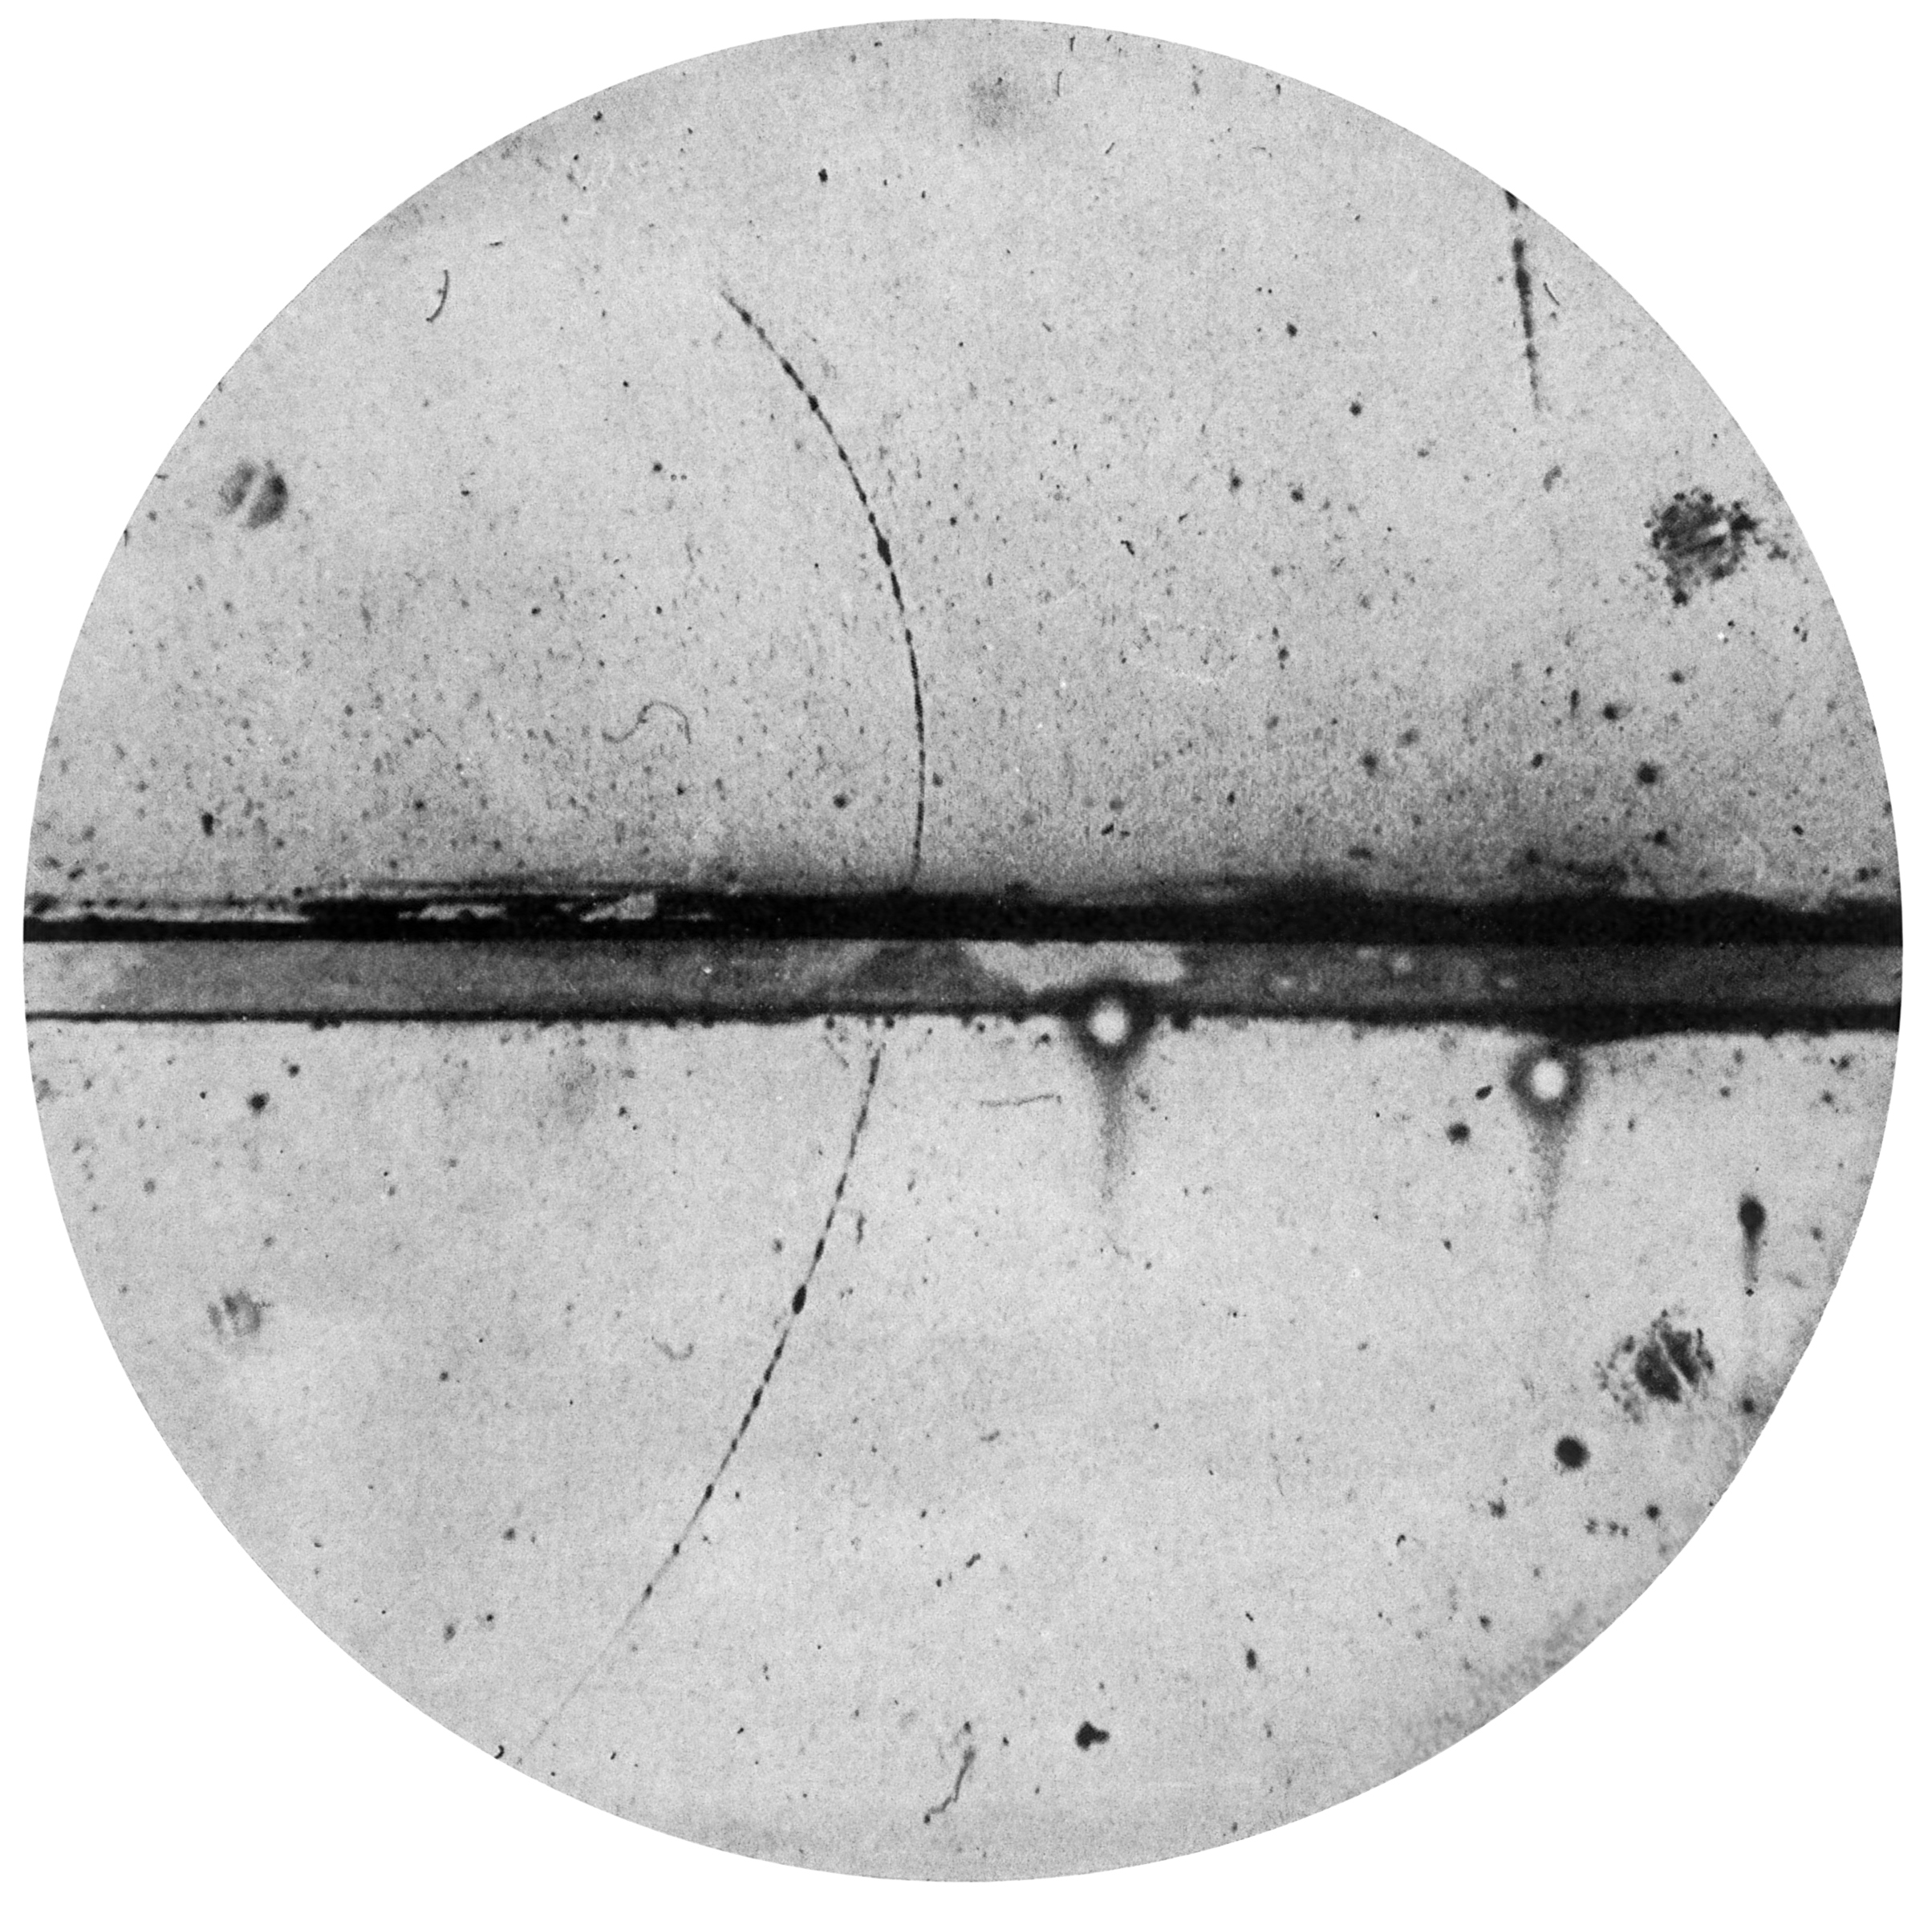
\includegraphics[width=0.25\textwidth]{PositronDiscovery.jpg}
\caption{\label{fig:pipe1} The trajectory of a sub-atomic particle through a cloud chamber.}
\end{figure}

\begin{enumerate}
\item The experimental result depicted in Fig. \ref{fig:pipe1} shows the trajectory of a sub-atomic particle that is revealed by a device called a \textit{cloud chamber.}  The particle bends to the \textit{left} after passing through a lead plate.  (a) The magnetic field is \textit{into the page.}  What is the sign of the charge of this particle? (b) It was later deduced that this particle had the mass of an elecron, from the radius of curvature.  Why is that strange? (c) Imagine the B-field had a strength of 0.05 T and the velocity of the paricle was $10^{6}$ m/s.  What was the force on the particle, and in what direction was the force?
\end{enumerate}

\end{document}